\chapter{Results} \label{chap:results}

This chapter reports the results of fitting the model of Chapter~\ref{chap:methodology} to the production
La Liga player--season dataset described in Chapter~\ref{chap:data_source}. Unless stated otherwise, every
number, table, and figure in this chapter comes from the constant-$\sigma_e$, $K^*=3$, Student-$t$ production
fit (Definition~\ref{def:additive}, $\boldsymbol\Sigma_a$ as in Definition~\ref{def:sigma_a}) --- the model
whose specification, identification, and rank selection were argued for in Chapter~\ref{chap:methodology}. The
one deliberate exception is \S\ref{sec:results-phi}, which resolves the fixed-vs-estimated $\phi$ question
(Remark~\ref{rem:phi}) using a pair of separate fits built specifically for that comparison.

\section{Model diagnostics and convergence}
\label{sec:results-diagnostics}

Table~\ref{tab:diagnostics-summary} summarises posterior convergence for the production fit, grouped by
parameter family. $\hat R$ and effective sample size are computed in the usual way from four parallel chains.
Three of the $144$ entries of $\boldsymbol\Lambda_a$ are excluded from the \emph{Lambda\_a} row: under the
lower-triangular, positive-diagonal constraint of \S\ref{sec:ltpd} these entries are fixed at exactly zero and
never sampled, so $\hat R$ is undefined for them (zero posterior variance) rather than poorly mixed.

\begin{table}[h]
\centering
\caption{Posterior convergence summary for the production fit ($K^*=3$), by parameter family. $\nu$ is the
Student-$t$ degrees of freedom (Definition~\ref{def:student_t}); $\boldsymbol\Lambda_a$, $\boldsymbol\Psi_a$
are the factor loadings and uniqueness (Definition~\ref{def:sigma_a}); $\boldsymbol\sigma_b,\boldsymbol\sigma_e$
are the season and residual scales. The LLt[1,10] row is the rotation-invariant bellwether check discussed
below.}
\label{tab:diagnostics-summary}

\begin{tabular}{lrlrr}
\toprule
Parameter & $N$ & ESS$_\text{bulk}$: median (min) & Max $\hat R$ & $N(\hat R{>}1.01)$\\
\midrule
$\boldsymbol\Lambda_a\boldsymbol\Lambda_a^\top$ (all entries) & 1176 & 603 (154) & 1.025 & 12\\
$d_1,d_2,d_3$ (eigenvalues) & 3 & 446 (216) & 1.004 & 0\\
$\boldsymbol\Lambda_a$ & 141 & 343 (75) & 1.032 & 36\\
$\nu$ & 1 & 2895 (2895) & 1.000 & 0\\
$\boldsymbol\psi_a$ & 48 & 1127 (546) & 1.005 & 0\\
$\boldsymbol\sigma_b$ & 48 & 1615 (1128) & 1.001 & 0\\
$\boldsymbol\sigma_e$ & 48 & 3983 (2548) & 1.002 & 0\\
\bottomrule
\end{tabular}

\end{table}

Convergence is excellent for the scalar and per-feature parameters: $\nu$, $\boldsymbol\psi_a$,
$\boldsymbol\sigma_b$, and $\boldsymbol\sigma_e$ all have $\hat R \leq 1.005$ and minimum bulk-ESS in the
hundreds to thousands. $\boldsymbol\Lambda_a$ itself mixes less cleanly (worst $\hat R = 1.014$, $4$ of the
$141$ sampled entries above the conventional $1.01$ threshold) --- but, as Remark~\ref{rem:ltpd_notinterp}
already anticipated, the raw loadings under the LT-PD identification constraint are an identification device,
not the object of substantive interest, so this is not by itself informative about whether the model has
recovered a genuine, stable shared-covariance structure. Proposition~\ref{prop:spectral_inv} gives the
rotation-invariant object that \emph{is} of substantive interest: the spectral decomposition of
$\hat{\boldsymbol\Lambda}_a\hat{\boldsymbol\Lambda}_a^\top$. Following that proposition, mixing was checked
directly on one representative entry of this rotation-invariant common-variance matrix, $[\boldsymbol\Lambda_a
\boldsymbol\Lambda_a^\top]_{1,10}$ (the goals--forward-passes pair, previously the single worst-mixing entry
identified during model development): $\hat{R} = 1.005$, bulk-ESS $\approx 237$, comfortably above the
$200$-draw threshold used throughout this chapter --- a clean pass, in contrast to the raw loadings'
noisier picture.

\begin{figure}[h]
\centering
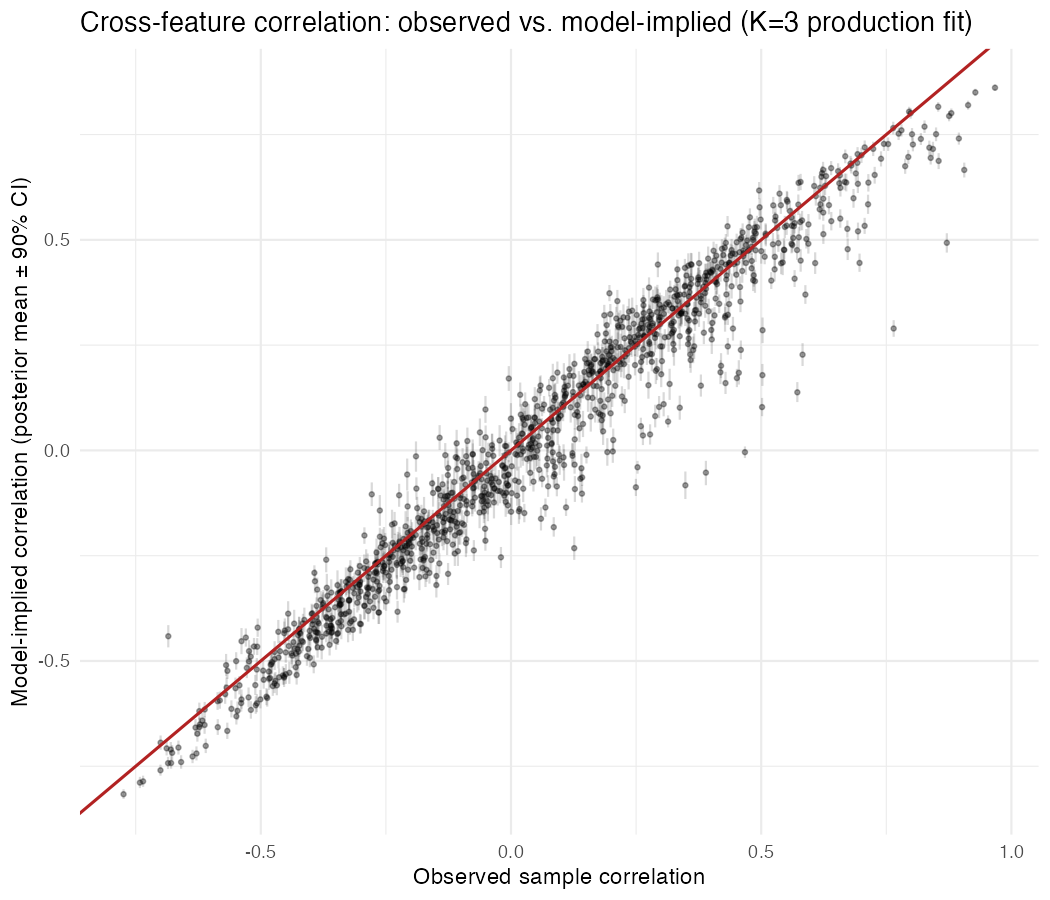
\includegraphics[width=0.85\textwidth]{images/40_correlation_ppc_scatter_k3.png}
\caption{Posterior predictive check: observed pairwise feature correlations vs. the model-implied correlation
$[\boldsymbol\Sigma_a]_{pq}/\sqrt{\mathrm{Var}(y_p)\mathrm{Var}(y_q)}$ (Proposition~\ref{prop:sigma_entries}),
posterior mean $\pm 90\%$ credible interval across $4{,}000$ draws. $r(\text{observed}, \text{model-implied}) =
0.975$.}
\label{fig:ppc-correlation}
\end{figure}

Figure~\ref{fig:ppc-correlation} checks whether the model reproduces the observed cross-feature correlation
structure: since $\boldsymbol\Sigma_b$ and $\boldsymbol\Sigma_e$ are diagonal by construction, every
model-implied off-diagonal correlation comes entirely from $\boldsymbol\Sigma_a = \boldsymbol\Lambda_a
\boldsymbol\Lambda_a^\top + \boldsymbol\Psi_a$. The near-perfect agreement ($r=0.975$) across all $\binom{48}{2}
= 1{,}128$ feature pairs indicates the three shared factors, plus feature-specific uniqueness, are jointly
sufficient to explain almost all of the pairwise dependence structure in the data --- direct support for the
low-rank modelling choice beyond the ELPD comparison of \S\ref{sec:results-rank}.

\begin{figure}[h]
\centering

\includegraphics[width=0.75\textwidth]{images/40_residual_distribution_check_k3.png}
\caption{Residual check: $y_{np} - \hat a_{i[n],p} - \hat b_{j[n],p}$ against $\mathcal{N}(0,\hat\sigma_{e,p})$
for six features (top-2 by ICC\_player, top-2 by ICC\_season, bottom-2 by combined ICC; \S\ref{sec:results-icc}).
The fitted noise model is Student-$t$, not Normal, so heavier-than-Normal tails here are expected, not a
misspecification.}
\label{fig:ppc-residual}
\end{figure}

\section{Rank selection: results}
\label{sec:results-rank}

Two separate questions were posed in \S\ref{sec:rank}: whether low-rank $\boldsymbol\Sigma_a$ is worth having
at all ($K=0$ vs.\ $K\geq1$), and, if so, which rank to use ($K^*$ among $K\geq1$). The evidence for the two
questions is qualitatively different, and this section reports them separately rather than blending them.

\paragraph{$K=0$ vs.\ $K\geq1$: decisive.} PSIS-LOO on the rebuilt production dataset ($N=4{,}586$, $P=48$)
gives $\Delta\mathrm{ELPD} = 5{,}820.2$ (SE $343.5$, $\approx 17$ standard errors) favouring the low-rank
$K^*=3$ model over the fully diagonal $K=0$ baseline. Pareto-$\hat k$ exceeds $0.5$ for the large majority of
observations under both models ($98.9\%$ diagonal, $99.3\%$ low-rank), so this magnitude should be read
directionally rather than as a precise variance estimate --- but a nearly-$17$-SE gap is not the kind of result
a directional caveat can reverse. Shared player-level covariance structure is real and worth modelling.

\paragraph{Choosing $K^*$ among $K \geq 1$: qualitative, per \S\ref{sec:rank_qualitative}.} Table~\ref{tab:rank-criteria}
recaps the three structural criteria across $K=2,3,4$ that \S\ref{sec:rank_qualitative} defined, since none of
the cross-validation screens discriminated among them (methodology.tex's condensed summary of that screen).

\begin{table}[h]
\centering
\caption{Criteria A--C across candidate ranks (\S\ref{sec:rank_qualitative}). Criterion A: last canonical
factor's share of $\bar{\boldsymbol\Lambda}_a\bar{\boldsymbol\Lambda}_a^\top$'s total variance. Criterion B:
count of features whose 90\% CI on that factor's loading excludes zero (of 48). Criterion C: mean fraction of
standardised residual cells exceeding the fit's own $t(\hat\nu)$-implied $\tau_{99}$ threshold.}
\label{tab:rank-criteria}

\begin{tabular}{rlllr}
\toprule
K & Last-PC share of LLt & Last-PC reliable loaders & Mean resid. > tau99 & nu\_hat\\
\midrule
2 & 30.8\% & 45/48 & 0.74\% & 4.88\\
3 & 10.5\% & 43/48 & 0.77\% & 4.90\\
4 & 7.1\% & 45/48 & 0.79\% & 4.95\\
\bottomrule
\end{tabular}

\end{table}

Criterion A mildly favours stopping at $K=3$ (the fourth factor's $7.1\%$ share is smaller than the third's
$10.5\%$, but the decline from $K{=}2\to3\to4$ is continuous, not a sharp drop to a noise floor). Criterion B
does not discriminate ($43/48$ at $K=3$ vs.\ $45/48$ at $K=4$ --- non-monotonic, so the fourth factor is, if
anything, as reliably identified as the third). Criterion C is flat and uninformative at this range (all three
ranks comfortably under the $1\%$ adequacy floor). Read honestly, this is a preference for the simpler model
under a still-shrinking-but-not-negligible fourth factor, not a clean reversal of the kind that separates $K=0$
from $K\geq1$. $K^*=3$ is retained on parsimony grounds and used throughout the rest of this chapter.

Figure~\ref{fig:holdout-elpd} shows the player-holdout cross-validation screen referenced above: consistent with
\S\ref{sec:rank_qualitative}'s framing, this is \emph{not} a clean K=3 win --- the base metric peaks at $K=6$ and the
minutes-scaled metric shows an elbow, not a sharp maximum, at $K=3$. It is included here for completeness and
transparency, not as evidence for $K^*=3$ on its own.

\begin{figure}[h]
\centering
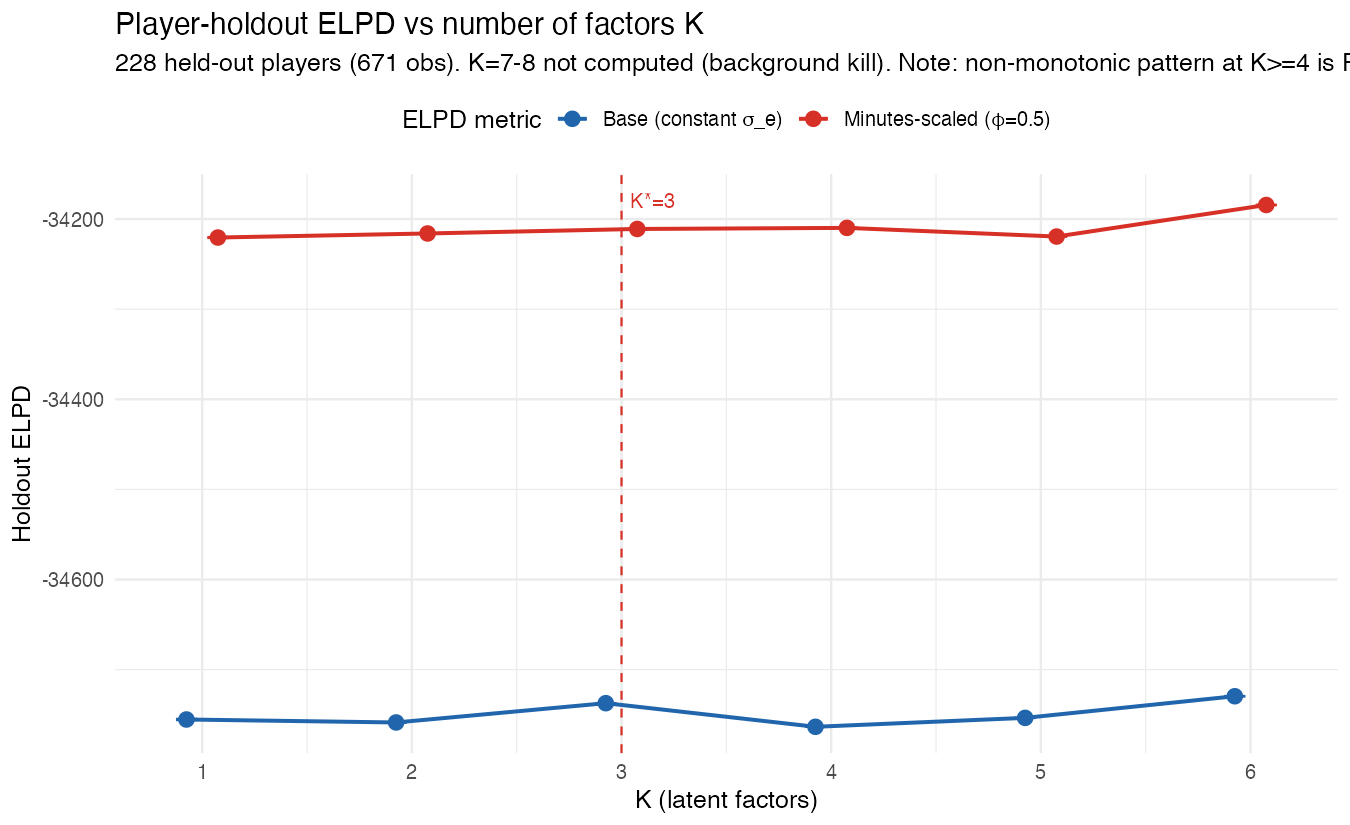
\includegraphics[width=0.75\textwidth]{images/32_player_holdout_elpd.png}
\caption{Player-holdout ELPD across $K=0,\ldots,8$ (base and minutes-scaled metrics, marginalized model,
$15\%$ player-level holdout). Neither metric produces a clean single maximum at $K=3$; both are best read as
broadly flat across $K\in\{2,\ldots,6\}$.}
\label{fig:holdout-elpd}
\end{figure}

\section{Resolving the observation-level variance scaling ($\phi$)}
\label{sec:results-phi}

Remark~\ref{rem:phi} left open whether the minutes-exposure scaling exponent $\phi$ in
Definition~\ref{def:phi} should be fixed or estimated, deferring the decision to this chapter. The motivation
for scaling at all came from a direct diagnostic on the constant-$\sigma_e$ fit: of the top-200 worst
standardised-residual cells, $48.9\%$ ($88/180$) came from the bottom quintile of playing time, against an
expected $20\%$ under no minutes effect (binomial $p < 4.4\times10^{-18}$) --- observations from low-minute
player-seasons are markedly under-fit by a model that treats residual variance as constant regardless of
exposure.

\begin{table}[h]
\centering
\caption{Resolving $\phi$: constant-$\sigma_e$ baseline vs.\ two minutes-scaled variants. "Low-minute
worst-cell share" repeats the diagnostic above, recomputed on each fit's own residuals.}
\label{tab:phi-comparison}
\input{tables/43_phi_comparison.tex}
\end{table}

Table~\ref{tab:phi-comparison} compares the constant-$\sigma_e$ production fit against two minutes-scaled
refits: $\phi$ fixed at the Poisson-rate value of $0.5$, and $\phi$ estimated freely. Both minutes-scaled
variants eliminate the low-minute over-representation almost entirely ($48.9\% \to 8.3\%$), confirming the
scaling addresses the diagnosed problem rather than merely reshuffling it. The estimated $\hat\phi = 0.366$
(90\% CI $[0.360, 0.373]$) is meaningfully below the fixed value of $0.5$: the data reject pure Poisson-rate
scaling in favour of a milder, super-Poisson exponent, consistent with some of a player's per-minute variance
being genuine heterogeneity (skill, role) rather than pure sampling noise that would vanish with more minutes.
Both scaled variants also push $\hat\nu$ higher (from $4.90$ to $5.67$--$5.98$): once exposure-driven
heteroscedasticity is accounted for, less of the remaining spread needs to be attributed to heavy tails.

\textbf{Verdict:} minutes-scaling with an estimated $\phi$ is the better-supported treatment for this data.
The rest of this chapter, however, continues to report results from the constant-$\sigma_e$ production fit
(stage 28): that is the fit all of the downstream infrastructure below (canonical loadings, archetypes,
similarity) was built against, and it is what Chapter~\ref{chap:methodology} describes as ``the model''
throughout. Re-deriving every subsequent result under the minutes-scaled variant is a natural extension, flagged
here rather than undertaken, since the qualitative substance of the loadings and similarity results is not
expected to change materially and the constant-$\sigma_e$ fit is the one already validated end-to-end.

\section{Variance decomposition: intraclass correlations}
\label{sec:results-icc}

Definition~\ref{def:icc} defines $\mathrm{ICC}_{a,p}$, $\mathrm{ICC}_{b,p}$, $\mathrm{ICC}_{e,p}$ as the share
of feature $p$'s total variance attributable to player, season, and residual, respectively.
Remark~\ref{rem:bayesian_icc} notes these are themselves posterior quantities, since every variance component
is sampled; Table~\ref{tab:icc-top15} reports posterior median and 90\% credible interval for the 15 features
with the highest player ICC (the full 48-feature table is given in Table~\ref{tab:icc-full}).

\begin{table}[h]
\centering
\caption{Player, season, and residual ICC (posterior median [90\% CI]) for the 15 features with the highest
player ICC.}
\label{tab:icc-top15}

\begin{tabular}{llll}
\toprule
Feature & ICC(player) & ICC(season) & ICC(resid.)\\
\midrule
recoveries & 0.89 [0.88, 0.90] & 0.01 [0.00, 0.02] & 0.11 [0.10, 0.11]\\
offensive duels & 0.87 [0.83, 0.90] & 0.04 [0.02, 0.09] & 0.08 [0.08, 0.09]\\
touch in box & 0.87 [0.86, 0.88] & 0.00 [0.00, 0.00] & 0.13 [0.12, 0.14]\\
forward passes & 0.87 [0.86, 0.88] & 0.00 [0.00, 0.01] & 0.13 [0.12, 0.14]\\
crosses & 0.85 [0.84, 0.86] & 0.01 [0.01, 0.03] & 0.13 [0.12, 0.14]\\
passes & 0.85 [0.83, 0.86] & 0.01 [0.00, 0.02] & 0.14 [0.13, 0.15]\\
long passes & 0.84 [0.82, 0.85] & 0.00 [0.00, 0.01] & 0.16 [0.15, 0.17]\\
xg shot & 0.83 [0.82, 0.84] & 0.00 [0.00, 0.00] & 0.17 [0.16, 0.18]\\
clearances & 0.83 [0.81, 0.85] & 0.02 [0.01, 0.04] & 0.15 [0.14, 0.16]\\
shots & 0.83 [0.81, 0.84] & 0.01 [0.00, 0.02] & 0.17 [0.16, 0.18]\\
lateral passes & 0.82 [0.80, 0.83] & 0.01 [0.01, 0.03] & 0.17 [0.16, 0.18]\\
progressive passes & 0.81 [0.77, 0.83] & 0.04 [0.02, 0.08] & 0.15 [0.14, 0.17]\\
aerial duels & 0.80 [0.74, 0.83] & 0.06 [0.03, 0.12] & 0.14 [0.13, 0.16]\\
dribbles & 0.80 [0.70, 0.84] & 0.11 [0.06, 0.21] & 0.10 [0.09, 0.11]\\
received pass & 0.78 [0.75, 0.80] & 0.03 [0.02, 0.08] & 0.18 [0.17, 0.20]\\
\bottomrule
\end{tabular}

\end{table}

Player identity dominates the variance of most features: all 15 features in Table~\ref{tab:icc-top15} have
$\mathrm{ICC}_{a} > 0.75$, and several exceed $0.85$ (recoveries, offensive duels, touch in box, forward
passes). Season ICC is small almost everywhere (typically under $0.05$), consistent with
\S\ref{sec:results-seasons}'s finding that season-level drift, while real, is a second-order effect relative to
player identity for most features. This is the quantitative counterpart to the qualitative claim motivating the
whole model (\S\ref{sec:covariance}): football performance profiles are substantially stable properties of the
player, not noise or pure context.

\begin{center}
\textbf{Table~\ref*{tab:icc-full}.} Full 48-feature ICC table (posterior median [90\% CI]).
\end{center}
\label{tab:icc-full}

\begin{longtable}{llll}
\toprule
Feature & ICC(player) & ICC(season) & ICC(resid.)\\
\midrule
recoveries & 0.89 [0.88, 0.90] & 0.01 [0.00, 0.02] & 0.11 [0.10, 0.11]\\
offensive duels & 0.87 [0.83, 0.90] & 0.04 [0.02, 0.09] & 0.08 [0.08, 0.09]\\
touch in box & 0.87 [0.86, 0.88] & 0.00 [0.00, 0.00] & 0.13 [0.12, 0.14]\\
forward passes & 0.87 [0.86, 0.88] & 0.00 [0.00, 0.01] & 0.13 [0.12, 0.14]\\
crosses & 0.85 [0.84, 0.86] & 0.01 [0.01, 0.03] & 0.13 [0.12, 0.14]\\
passes & 0.85 [0.83, 0.86] & 0.01 [0.00, 0.02] & 0.14 [0.13, 0.15]\\
long passes & 0.84 [0.82, 0.85] & 0.00 [0.00, 0.01] & 0.16 [0.15, 0.17]\\
xg shot & 0.83 [0.82, 0.84] & 0.00 [0.00, 0.00] & 0.17 [0.16, 0.18]\\
clearances & 0.83 [0.81, 0.85] & 0.02 [0.01, 0.04] & 0.15 [0.14, 0.16]\\
shots & 0.83 [0.81, 0.84] & 0.01 [0.00, 0.02] & 0.17 [0.16, 0.18]\\
lateral passes & 0.82 [0.80, 0.83] & 0.01 [0.01, 0.03] & 0.17 [0.16, 0.18]\\
progressive passes & 0.81 [0.77, 0.83] & 0.04 [0.02, 0.08] & 0.15 [0.14, 0.17]\\
aerial duels & 0.80 [0.74, 0.83] & 0.06 [0.03, 0.12] & 0.14 [0.13, 0.16]\\
dribbles & 0.80 [0.70, 0.84] & 0.11 [0.06, 0.21] & 0.10 [0.09, 0.11]\\
received pass & 0.78 [0.75, 0.80] & 0.03 [0.02, 0.08] & 0.18 [0.17, 0.20]\\
interceptions & 0.77 [0.71, 0.80] & 0.06 [0.03, 0.12] & 0.17 [0.16, 0.19]\\
back passes & 0.77 [0.75, 0.78] & 0.01 [0.00, 0.02] & 0.22 [0.21, 0.24]\\
successful passes & 0.76 [0.73, 0.78] & 0.03 [0.01, 0.06] & 0.21 [0.19, 0.22]\\
passes to final third & 0.76 [0.74, 0.78] & 0.02 [0.01, 0.04] & 0.22 [0.21, 0.24]\\
shot assists & 0.74 [0.72, 0.76] & 0.01 [0.01, 0.03] & 0.24 [0.23, 0.26]\\
fouls suffered & 0.73 [0.71, 0.75] & 0.02 [0.01, 0.05] & 0.25 [0.23, 0.26]\\
progressive run & 0.72 [0.68, 0.75] & 0.04 [0.02, 0.09] & 0.23 [0.21, 0.25]\\
opponent half recoveries & 0.69 [0.67, 0.71] & 0.01 [0.00, 0.01] & 0.31 [0.29, 0.33]\\
head shots & 0.68 [0.66, 0.70] & 0.00 [0.00, 0.00] & 0.32 [0.30, 0.34]\\
defensive duels & 0.68 [0.61, 0.71] & 0.10 [0.05, 0.19] & 0.23 [0.20, 0.25]\\
aerial duels won & 0.66 [0.64, 0.68] & 0.01 [0.00, 0.01] & 0.33 [0.31, 0.35]\\
losses & 0.64 [0.57, 0.68] & 0.09 [0.05, 0.19] & 0.26 [0.23, 0.28]\\
dribbles against & 0.64 [0.56, 0.69] & 0.14 [0.08, 0.25] & 0.22 [0.19, 0.24]\\
goals & 0.64 [0.62, 0.66] & 0.00 [0.00, 0.00] & 0.36 [0.34, 0.38]\\
key passes & 0.63 [0.61, 0.65] & 0.00 [0.00, 0.01] & 0.36 [0.34, 0.38]\\
xg assist & 0.63 [0.61, 0.65] & 0.01 [0.00, 0.01] & 0.36 [0.34, 0.38]\\
fouls & 0.62 [0.59, 0.64] & 0.03 [0.01, 0.07] & 0.35 [0.32, 0.37]\\
loose ball duels & 0.60 [0.51, 0.65] & 0.15 [0.08, 0.28] & 0.25 [0.21, 0.27]\\
accelerations & 0.60 [0.51, 0.65] & 0.14 [0.08, 0.26] & 0.26 [0.22, 0.29]\\
shots blocked & 0.59 [0.56, 0.61] & 0.01 [0.01, 0.03] & 0.40 [0.38, 0.42]\\
sliding tackles & 0.56 [0.49, 0.61] & 0.12 [0.06, 0.23] & 0.32 [0.28, 0.35]\\
through passes & 0.50 [0.42, 0.54] & 0.14 [0.08, 0.27] & 0.36 [0.31, 0.40]\\
own half losses & 0.49 [0.46, 0.51] & 0.02 [0.01, 0.06] & 0.49 [0.46, 0.51]\\
offensive duels won & 0.47 [0.45, 0.50] & 0.02 [0.01, 0.05] & 0.50 [0.48, 0.53]\\
pressing duels & 0.44 [0.33, 0.52] & 0.31 [0.20, 0.48] & 0.25 [0.19, 0.29]\\
smart passes & 0.40 [0.28, 0.49] & 0.44 [0.30, 0.60] & 0.17 [0.12, 0.21]\\
dangerous own half losses & 0.39 [0.36, 0.42] & 0.01 [0.01, 0.03] & 0.60 [0.57, 0.62]\\
successful progressive passes & 0.39 [0.34, 0.42] & 0.09 [0.05, 0.19] & 0.52 [0.46, 0.56]\\
yellow cards & 0.36 [0.33, 0.39] & 0.02 [0.01, 0.05] & 0.61 [0.58, 0.65]\\
defensive duels won & 0.36 [0.29, 0.40] & 0.20 [0.11, 0.34] & 0.44 [0.36, 0.50]\\
dangerous opponent half recoveries & 0.35 [0.32, 0.38] & 0.01 [0.00, 0.02] & 0.64 [0.62, 0.67]\\
assists & 0.33 [0.30, 0.35] & 0.01 [0.00, 0.02] & 0.66 [0.64, 0.69]\\
successful dribbles & 0.30 [0.27, 0.33] & 0.01 [0.01, 0.04] & 0.69 [0.66, 0.72]\\
\bottomrule
\end{longtable}


\section{Canonical factor directions and their football interpretation}
\label{sec:results-canonical}

Raw $\boldsymbol\Lambda_a$, fitted under the LT-PD constraint of \S\ref{sec:ltpd}, is an identification device
and should not be interpreted directly (Remark~\ref{rem:ltpd_notinterp}). Following
Definition~\ref{def:pca_postproc}, canonical factor directions are instead obtained by eigendecomposing the
common-variance matrix $\bar{\boldsymbol\Lambda}_a\bar{\boldsymbol\Lambda}_a^\top$
(Proposition~\ref{prop:spectral_inv} shows this is invariant to the identification constraint used at fit
time).

\begin{table}[h]
\centering
\caption{Variance shares of the three canonical factors, for the common-variance matrix
$\bar{\boldsymbol\Lambda}_a\bar{\boldsymbol\Lambda}_a^\top$ and for total player variance
$\bar{\boldsymbol\Sigma}_a = \bar{\boldsymbol\Lambda}_a\bar{\boldsymbol\Lambda}_a^\top + \bar{\boldsymbol\Psi}_a$.
The gap between the two columns for each PC is the share absorbed by feature-specific uniqueness
$\boldsymbol\Psi_a$ instead of the shared factors.}
\label{tab:pca-variance-shares}
\begin{tabular}{lcc}
\toprule
Canonical factor & Share of $\bar{\boldsymbol\Lambda}_a\bar{\boldsymbol\Lambda}_a^\top$ & Share of $\bar{\boldsymbol\Sigma}_a$ \\
\midrule
PC1 & 61.8\% & 45.6\% \\
PC2 & 27.7\% & 20.7\% \\
PC3 & 10.5\% & 8.1\% \\
\bottomrule
\end{tabular}
\end{table}

Roughly a quarter of total player-level variance sits in $\boldsymbol\Psi_a$ rather than the three shared
factors (Table~\ref{tab:pca-variance-shares}) --- a meaningful idiosyncratic component that
\S\ref{sec:results-similarity} returns to directly.

\begin{figure}[h]
\centering

\includegraphics[width=0.9\textwidth]{images/31_pca_loading_ci_plot.png}
\caption{Canonical factor loadings with 90\% credible intervals. Solid points/intervals: reliable loaders
(CI excludes zero). PC1: defensive work-rate (positive) vs.\ attacking output (negative). PC2: pass-based /
technical (positive) vs.\ aerial / physical (negative). PC3: possession quality (positive) vs.\ wide / direct
play (negative).}
\label{fig:pca-loadings}
\end{figure}

Table~\ref{tab:canonical-pc1}--\ref{tab:canonical-pc3} list the most reliable loaders (90\% CI excludes zero)
for each canonical factor.

\begin{table}[h]
\centering
\caption{Top reliable loaders, canonical factor PC1 (defensive work-rate vs.\ attacking output).}
\label{tab:canonical-pc1}

\begin{tabular}{lll}
\toprule
Feature & Group & Loading\\
\midrule
recoveries & Defending & 0.90 [0.85, 0.95]\\
forward passes & Passing volume & 0.82 [0.76, 0.87]\\
interceptions & Defending & 0.81 [0.76, 0.86]\\
offensive duels & Dueling & -0.80 [-0.86, -0.74]\\
touch in box & Attacking output & -0.80 [-0.85, -0.75]\\
shots & Attacking output & -0.79 [-0.84, -0.75]\\
clearances & Defending & 0.78 [0.72, 0.83]\\
long passes & Passing volume & 0.78 [0.72, 0.83]\\
\bottomrule
\end{tabular}

\end{table}

\begin{table}[h]
\centering
\caption{Top reliable loaders, canonical factor PC2 (technical/pass-based vs.\ aerial/physical).}
\label{tab:canonical-pc2}

\begin{tabular}{lll}
\toprule
Feature & Group & Loading\\
\midrule
received pass & Passing volume & 0.65 [0.63, 0.68]\\
passes & Passing volume & 0.63 [0.60, 0.65]\\
back passes & Passing volume & 0.63 [0.62, 0.63]\\
aerial duels & Dueling & -0.59 [-0.60, -0.58]\\
shot assists & Passing volume & 0.59 [0.58, 0.60]\\
head shots & Attacking output & -0.59 [-0.60, -0.58]\\
crosses & Passing volume & 0.56 [0.55, 0.57]\\
progressive passes & Passing volume & 0.55 [0.53, 0.56]\\
\bottomrule
\end{tabular}

\end{table}

\begin{table}[h]
\centering
\caption{Top reliable loaders, canonical factor PC3 (possession quality vs.\ wide/direct play).}
\label{tab:canonical-pc3}

\begin{tabular}{lll}
\toprule
Feature & Group & Loading\\
\midrule
successful passes & Passing quality & 0.56 [0.54, 0.58]\\
crosses & Passing volume & -0.48 [-0.50, -0.45]\\
dribbles against & Defending & -0.46 [-0.48, -0.44]\\
defensive duels & Dueling & -0.44 [-0.46, -0.42]\\
lateral passes & Passing volume & 0.43 [0.42, 0.45]\\
received pass & Passing volume & 0.41 [0.40, 0.43]\\
passes & Passing volume & 0.36 [0.34, 0.38]\\
head shots & Attacking output & 0.33 [0.31, 0.36]\\
\bottomrule
\end{tabular}

\end{table}

\paragraph{Reconciling three factors with the earlier eleven.} Chapter~\ref{chap:background} reported an
eleven-factor exploratory solution from classical factor analysis of the raw, unpartitioned player--season
matrix. Remark~\ref{rem:k_not_comparable} explains why $K^*=3$ is not in tension with that finding: the
classical analysis describes the total covariance of $\mathbf y_n$, in which any two features that co-vary for
\emph{any} reason --- shared player skill, a league-wide tactical shift, or coincidental season drift ---
contribute jointly to the recovered factor count. $\boldsymbol\Sigma_a$, by contrast, is the covariance of what
is left of a player \emph{after} season-level drift and observation noise are subtracted out
(Definition~\ref{def:additive}); a smaller $K$ for that narrower object is the expected consequence of
conditioning on more structure, not a contradiction between the two analyses. As that remark itself notes, this
explanation has not been independently validated (e.g.\ by refitting the classical FA on a player-only,
season-averaged version of the data) and should be read as an argument for the direction of the discrepancy,
not a demonstrated equivalence.

\section{Player archetypes}
\label{sec:results-archetypes}

Projecting each player's posterior-mean effect onto the three canonical directions gives every player a
position in a $3$-dimensional style space. $k$-means clustering ($k=5$) on the (PC1, PC2) plane recovers five
groups that align closely with recognisable positional roles once ordered by PC1 (Figure~\ref{fig:archetype-scatter}):
Forwards, Attacking midfielders, Midfielders, Defensive midfielders, and Centre backs, running from the most
attacking to the most defensive end of PC1.

\begin{figure}[h]
\centering

\includegraphics[width=0.85\textwidth]{images/29_factor_score_scatter_clustered.png}
\caption{Player archetypes: PC1 vs.\ PC2 for all 1{,}529 outfield players, coloured by $k$-means cluster
($k=5$). Labelled points are the most extreme players per cluster on PC1/PC2.}
\label{fig:archetype-scatter}
\end{figure}

Tables~\ref{tab:archetype-pc1}--\ref{tab:archetype-pc3} list the most extreme players on each canonical
factor.

\begin{table}[h]
\centering
\caption{Top and bottom 8 players on PC1 (defensive work-rate vs.\ attacking output).}
\label{tab:archetype-pc1}

\begin{tabular}{llr}
\toprule
Player & Direction & Score\\
\midrule
Andreu Fontàs & top & 6.87\\
J. Mascherano & top & 6.59\\
M. Gabbia & top & 6.36\\
Aythami Artiles & top & 6.35\\
Zé Castro & top & 6.35\\
Antonio Amaya & top & 6.25\\
Gerard Piqué & top & 6.23\\
A. Ba & top & 6.00\\
Vinícius Júnior & bottom & -8.35\\
Neymar & bottom & -8.32\\
K. Mbappé & bottom & -8.21\\
L. Messi & bottom & -7.82\\
G. Mikautadze & bottom & -7.49\\
Cristiano Ronaldo & bottom & -7.46\\
Maroan Sannadi & bottom & -7.40\\
N. Amrabat & bottom & -7.40\\
\bottomrule
\end{tabular}

\end{table}

\begin{table}[h]
\centering
\caption{Top and bottom 8 players on PC2 (technical/pass-based vs.\ aerial/physical).}
\label{tab:archetype-pc2}

\begin{tabular}{llr}
\toprule
Player & Direction & Score\\
\midrule
C. Stuani & top & 7.09\\
A. Véliz & top & 7.07\\
Chris Ramos & top & 6.92\\
A. Budimir & top & 6.43\\
Manucho Gonçalves & top & 6.39\\
E. Boateng & top & 6.17\\
S. Okazaki & top & 6.11\\
Y. En-Nesyri & top & 6.09\\
Xavi & bottom & -7.40\\
L. Messi & bottom & -7.38\\
Andrés Iniesta & bottom & -6.84\\
J. Rodríguez & bottom & -6.82\\
Neymar & bottom & -6.74\\
É. Banega & bottom & -6.49\\
Dani Alves & bottom & -6.27\\
T. Kroos & bottom & -6.21\\
\bottomrule
\end{tabular}

\end{table}

\begin{table}[h]
\centering
\caption{Top and bottom 8 players on PC3 (possession quality vs.\ wide/direct play).}
\label{tab:archetype-pc3}

\begin{tabular}{llr}
\toprule
Player & Direction & Score\\
\midrule
Iván Alejo & top & 5.00\\
Juan Iglesias & top & 4.55\\
O. Vranješ & top & 4.46\\
Houboulang Mendes & top & 4.20\\
A. Aznou & top & 4.10\\
Miguel Llambrich & top & 3.97\\
Rubén Sánchez & top & 3.97\\
Davinchi & top & 3.85\\
L. Messi & bottom & -6.07\\
Xavi & bottom & -5.82\\
M. Pjanić & bottom & -5.46\\
Cristiano Ronaldo & bottom & -4.92\\
K. Benzema & bottom & -4.52\\
T. Kroos & bottom & -4.13\\
Arthur & bottom & -3.96\\
Andrés Iniesta & bottom & -3.95\\
\bottomrule
\end{tabular}

\end{table}

\section{Season profiles}
\label{sec:results-seasons}

Consistent with Table~\ref{tab:icc-top15}, season ICC is small for almost every feature --- but small does not
mean zero, and group-averaged season effects reveal coherent league-wide drift over the twelve seasons in the
data (Figure~\ref{fig:season-trends}).

\begin{figure}[h]
\centering

\includegraphics[width=0.95\textwidth]{images/33_season_group_trends.png}
\caption{Group-averaged posterior-mean season effects $\hat{\mathbf b}_j$, by feature group, 2011/12--2022/23.}
\label{fig:season-trends}
\end{figure}

\begin{figure}[h]
\centering

\includegraphics[width=0.85\textwidth]{images/36_season_top5_profiles.png}
\caption{The five features with the largest peak-to-trough range in $\hat{\mathbf b}_j$ across seasons. Smart
passes shows the largest range (2.4$\sigma$), on a falling trend consistent with a tactical shift away from
risk-laden through-balls over the sample period.}
\label{fig:season-top5}
\end{figure}

\section{Player similarity --- a fully Bayesian style/level decomposition}
\label{sec:results-similarity}

This section takes up, in depth, the question the Introduction posed at the outset: what does it mean for two
players to be ``similar,'' and can a player be stylistically similar to an outlier without matching their
output?

\subsection{Motivation: separating style from level}

The model's own covariance structure already gives a principled way to make this split. Recall
(Definition~\ref{def:sigma_a}, and the non-centred form of \S\ref{sec:noncentred}) that the player effect
decomposes as
\[
\mathbf a_i = \boldsymbol\Lambda_a\boldsymbol\eta_i + \boldsymbol\psi_a \odot \mathbf z_{u,i},
\]
a \emph{shared} component driven by the $K^*=3$ canonical factors, and an \emph{idiosyncratic} component that
those factors do not explain. \textbf{Style} is naturally read off the shared component: a player's position in
the $3$-dimensional canonical factor space, $\mathbf f_i$ (Definition~\ref{def:pca_postproc}), the same
coordinates used for the archetype clustering of \S\ref{sec:results-archetypes}. \textbf{Level} is naturally
read off the specific output features that shared style position does not by itself pin down --- here, goals
and expected goals per shot.

Two players can therefore be \emph{style-close} (near-identical $\mathbf f_i$) while being \emph{level-far}
(very different modelled goal output). That is the model-native version of ``can a player be stylistically
similar to an outlier without matching their production'': yes, and the mechanism is explicit rather than
asserted. It also explains why a true generational outlier is unlikely to have a perfect twin --- their
outlier-ness lives disproportionately in $\boldsymbol\psi_a \odot \mathbf z_{u,i}$, the part of their identity
that is, by construction, not shared with anyone else. Matching someone's shared style is achievable; matching
both their style and their most idiosyncratic output is structurally much less likely.

\emph{A note on scope}: the dataset is La Liga only, 2011/12--2022/23 (Chapter~\ref{chap:data_source}). A player like
Erling Haaland, who has never played in this league, is not in this analysis. He is a useful illustration of
the ``generational outlier'' idea in the abstract, never a literal query target here --- every concrete example
below uses an actual in-sample player as the stand-in.

\subsection{Classical point-estimate baseline}

Before the fully Bayesian treatment, a simpler point-estimate version: standardise each player's three PCA
scores and compute Euclidean distance. This is a single number per pair, with no posterior uncertainty on the
distance itself. Under this metric, Messi's nearest neighbour is Neymar (distance $1.74$) and Ramos's is Piqué
(distance $0.16$) --- both plausible, well-known pairings. Figure~\ref{fig:radar-examples} shows what such a
pairing looks like at the level of individual features, using the percentile radar of
\S\ref{sec:results-archetypes}'s eight feature groups. The next two subsections show what changes when the
same similarity question is asked with full posterior uncertainty attached.

\begin{figure}[h]
\centering

\includegraphics[width=0.32\textwidth]{images/37_radar_messi_neymar.png}\hfill

\includegraphics[width=0.32\textwidth]{images/37_radar_ramos_pique.png}\hfill
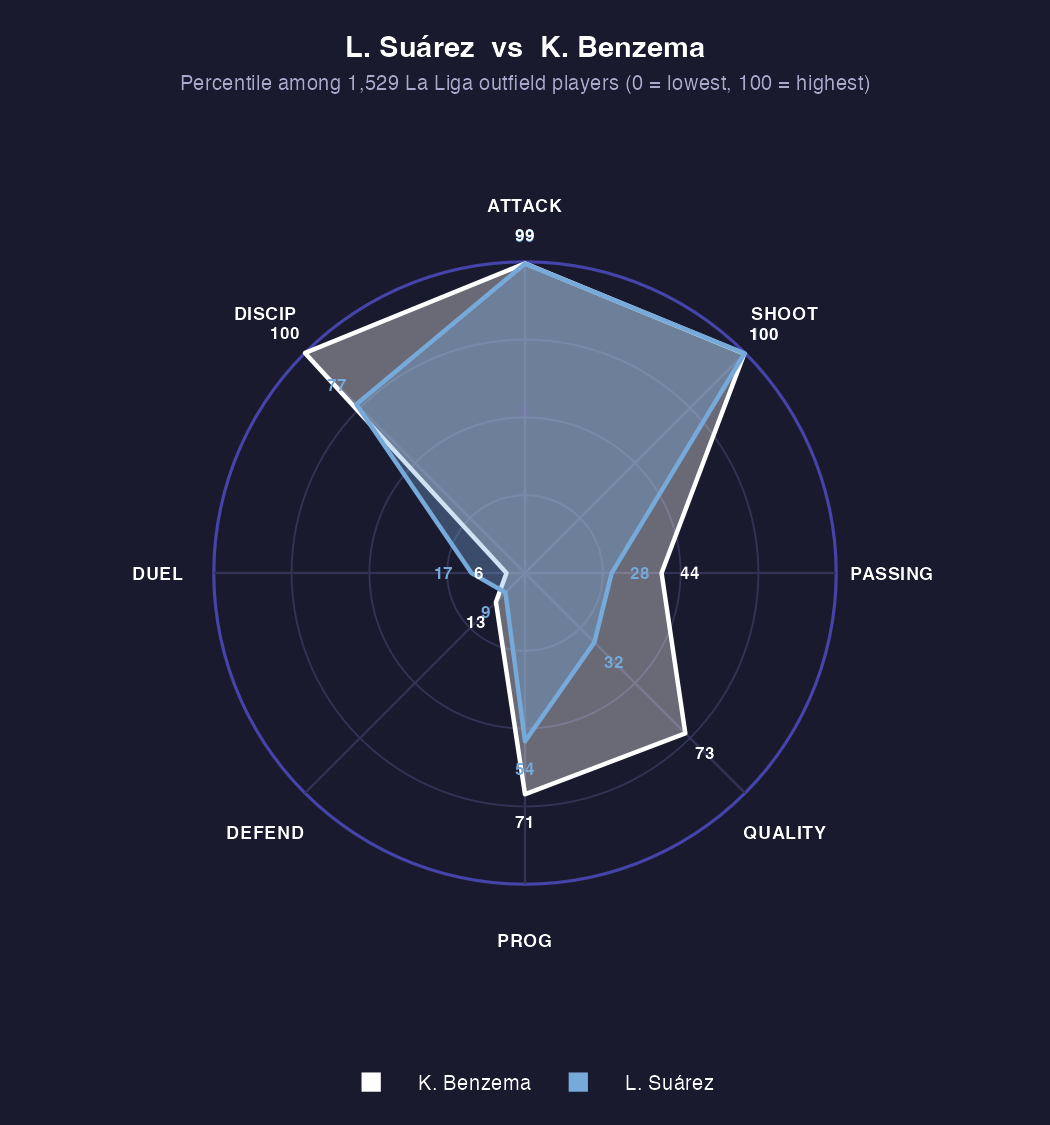
\includegraphics[width=0.32\textwidth]{images/37_radar_suarez_benzema.png}
\caption{Percentile radar comparisons (percentile among all 1,529 outfield players) for three of the
point-estimate pairings above. Messi--Neymar: the closest pair overall, near-identical across all eight
groups. Ramos--Piqué: two elite centre-backs, Ramos leading Dueling and Piqué leading Passing quality --- the
pairing \S\ref{sec:results-similarity} shows is actually a four-way statistical tie once posterior uncertainty
is accounted for. Suárez--Benzema: contrasting centre-forward profiles, relevant to the Benzema case study
below.}
\label{fig:radar-examples}
\end{figure}

\subsection{A fully Bayesian similarity score}

Rather than compute the archetype distance once, on posterior means, it is recomputed \emph{per posterior
draw}: for each draw $s$, standardise $\mathbf f_i^{(s)}$ across all players and compute the Euclidean distance
to a query player. This gives a posterior mean and 90\% credible interval on the style distance itself, plus a
stability statistic --- the fraction of draws in which a given candidate is the single closest player, not just
one of several close ones. The same per-draw treatment applied to $A[i,\text{goals}]$ and $A[i,\text{xG}]$
gives an equivalent posterior distribution for the level gap.

This was run for 17 named players, deliberately chosen to span all five archetype clusters of
\S\ref{sec:results-archetypes} rather than attacking players alone: Messi, Cristiano Ronaldo, Neymar, Luis
Suárez, Karim Benzema, Antoine Griezmann, and Iago Aspas (attacking midfielders/forwards); Sergio Busquets and
Saúl Ñíguez (defensive midfielders); Luka Modrić, Dani Carvajal, and Koke (midfielders); Sergio Ramos, Gerard
Piqué, José Giménez, and Íñigo Martínez (centre backs); and Iñaki Williams (forward).

\begin{figure}[h]
\centering
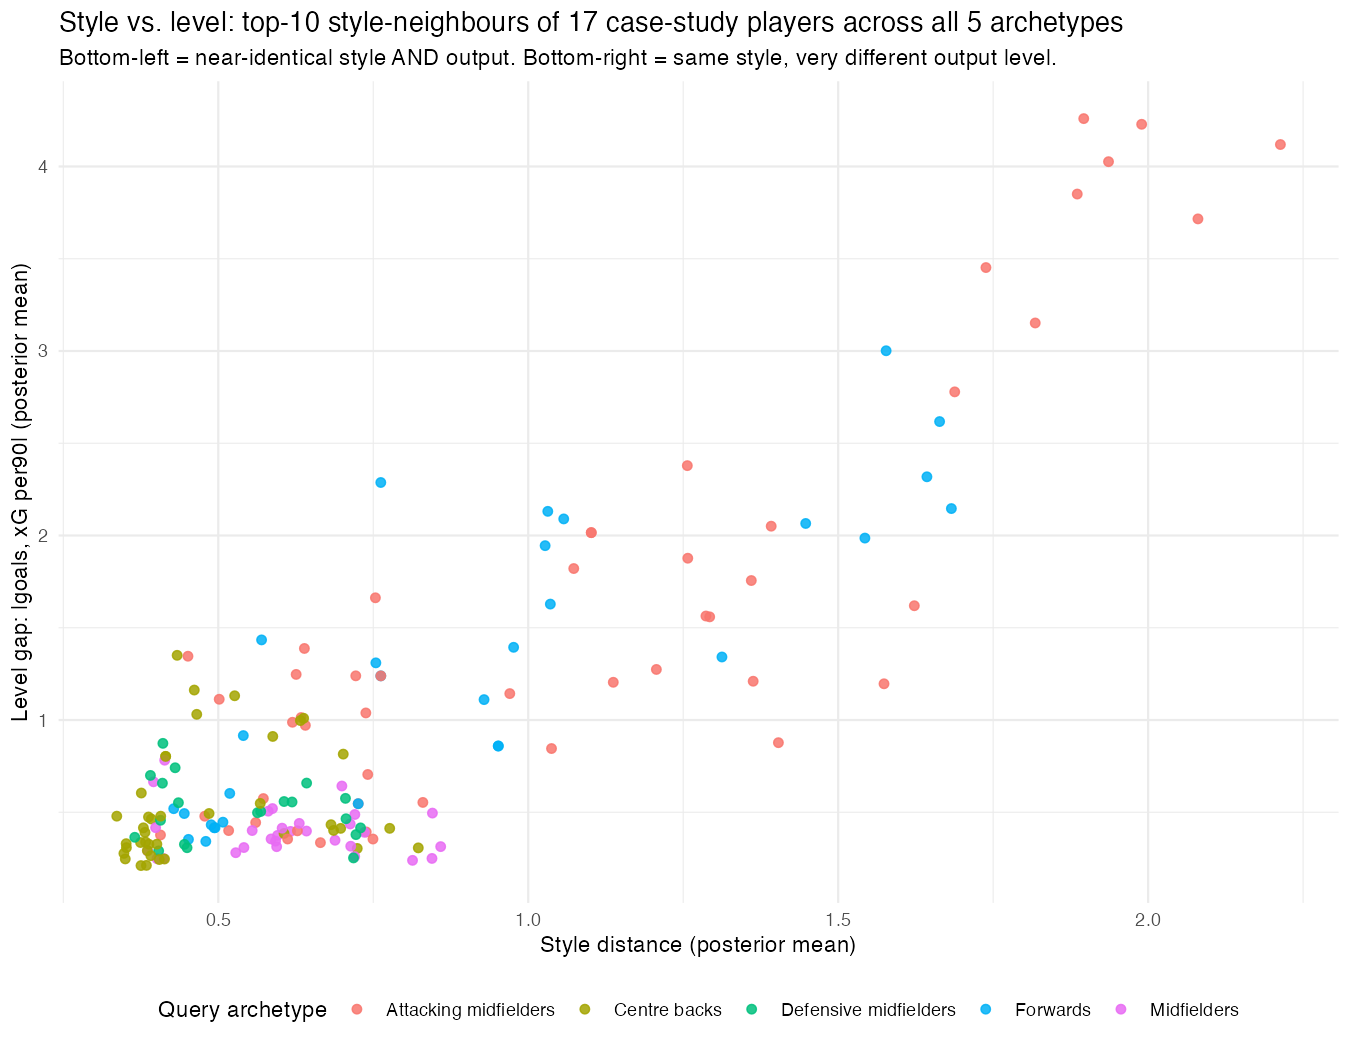
\includegraphics[width=0.9\textwidth]{images/42_style_vs_level_scatter_extended.png}
\caption{Style distance vs.\ level gap for the top-10 style-neighbours of all 17 case-study players, coloured
by query archetype. Points toward the bottom-right are the clearest examples of ``same shape, different output
level'' --- a stylistic twin at a different tier.}
\label{fig:style-vs-level-extended}
\end{figure}

\paragraph{Benzema's closest style-neighbour is not Ronaldo.} The classical point-estimate metric would rank
Cristiano Ronaldo first for Benzema (they were team-mates, and a blended metric partly reflects shared
context/service as well as shared style). The draw-level treatment instead makes S.\ Jovetić the modal closest
match ($39\%$ of draws), with Ronaldo a clear second ($25\%$) --- and, more to the point, Ronaldo carries the
\emph{largest} level gap of Benzema's four closest style-neighbours. Read together: even Benzema, an elite
striker whose shape is genuinely close to Ronaldo's, cannot close the level gap to him. Ronaldo's idiosyncratic
scoring output separates him from his closest stylistic peers, not just from the pool at large --- a direct,
data-driven instance of the mechanism described above.

\paragraph{Ramos's closest neighbour is a near four-way statistical tie.} The classical point estimate placed
Javi García first, ahead of Gerard Piqué, by a margin of $0.003$ ($0.161$ vs.\ $0.164$). The draw-level
treatment shows four centre-backs --- Piqué, Umtiti, García, Mathieu --- within a similar style-distance range,
each the single closest neighbour in only $16$--$24\%$ of draws. Piqué is the modal pick, consistent with the
well-known Ramos--Piqué pairing, but the honest statement is a four-way toss-up, not a confident single answer.
A point estimate cannot distinguish ``clearly the closest neighbour'' from ``one of several statistically
indistinguishable candidates''; here, the two cases look identical until the posterior draws are examined
individually.

Figure~\ref{fig:posterior-clouds} makes both findings visible directly, rather than through a single
distance-plus-percentage summary. A player's position in style space is not a point --- it is a posterior
\emph{cloud}, and whether two players are confidently close or only ambiguously close is a visual fact about
how much their clouds overlap.

\begin{figure}[h]
\centering
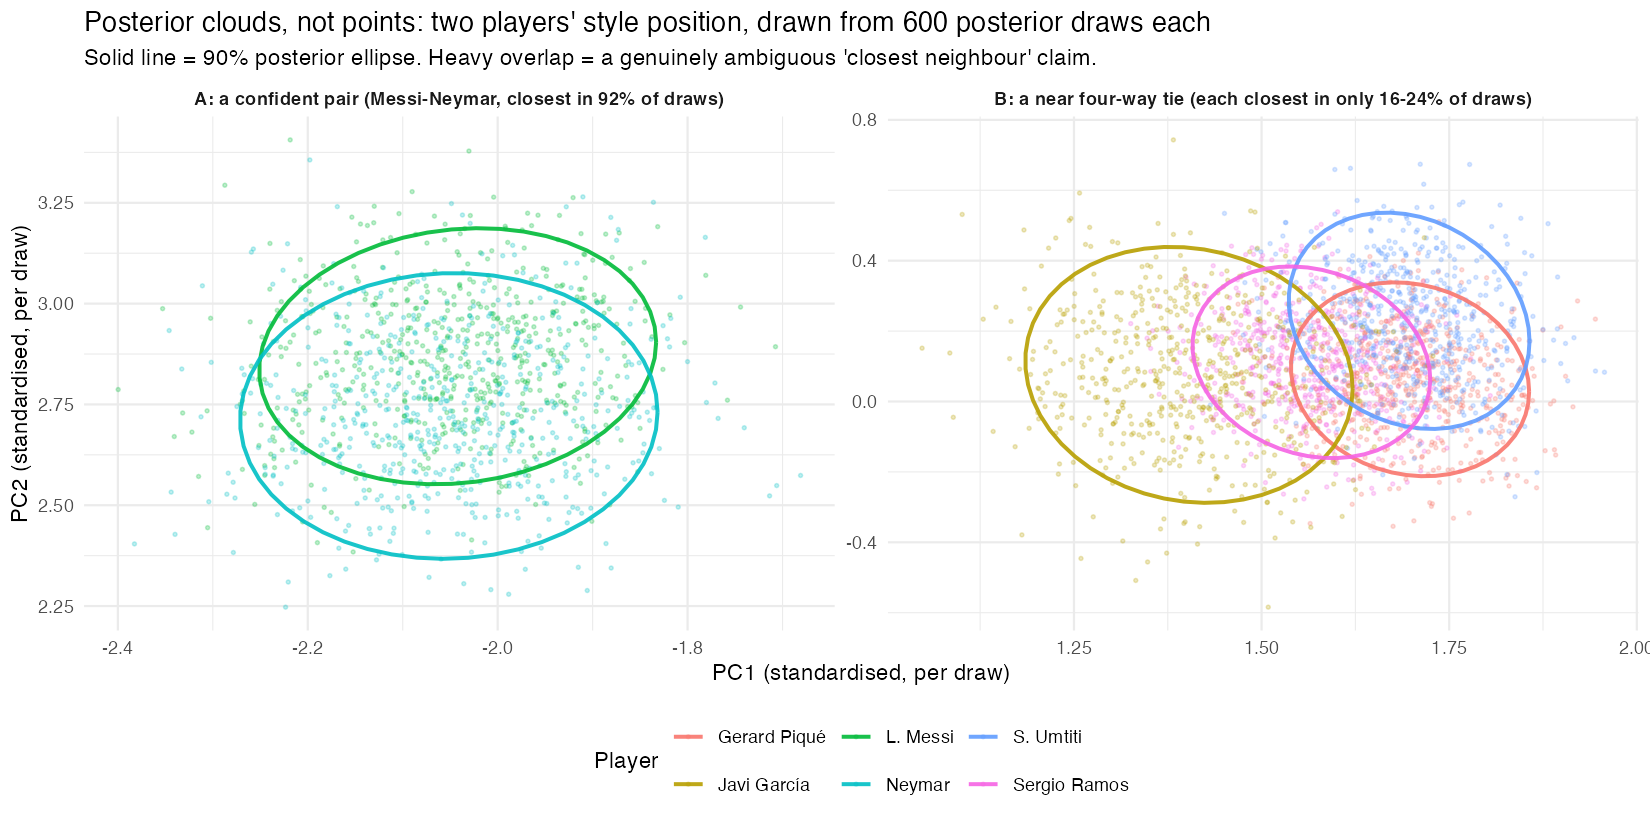
\includegraphics[width=\textwidth]{images/44_posterior_clouds.png}
\caption{Posterior clouds (600 subsampled draws, 90\% posterior ellipse) for the two cases above. Panel A:
Messi and Neymar's clouds are almost entirely overlapping, visualising the $92\%$ draw-level stability of that
pairing. Panel B: Ramos, Piqué, Umtiti, and Javi García's clouds overlap each other substantially and
unevenly --- the visual counterpart of a genuine four-way tie, not a confident single answer.}
\label{fig:posterior-clouds}
\end{figure}

\subsection{Population-level reliability}

The case studies above are all well-known, heavily-observed players. A natural question is whether the
stability of the ``closest neighbour'' claim generalises, or is itself a property of being a well-documented
star. To check this, the same per-draw procedure was run for a random sample of 150 players (not selected for
prominence), computing, for each, the posterior stability of \emph{their own} top-1 style-neighbour.

\begin{figure}[h]
\centering
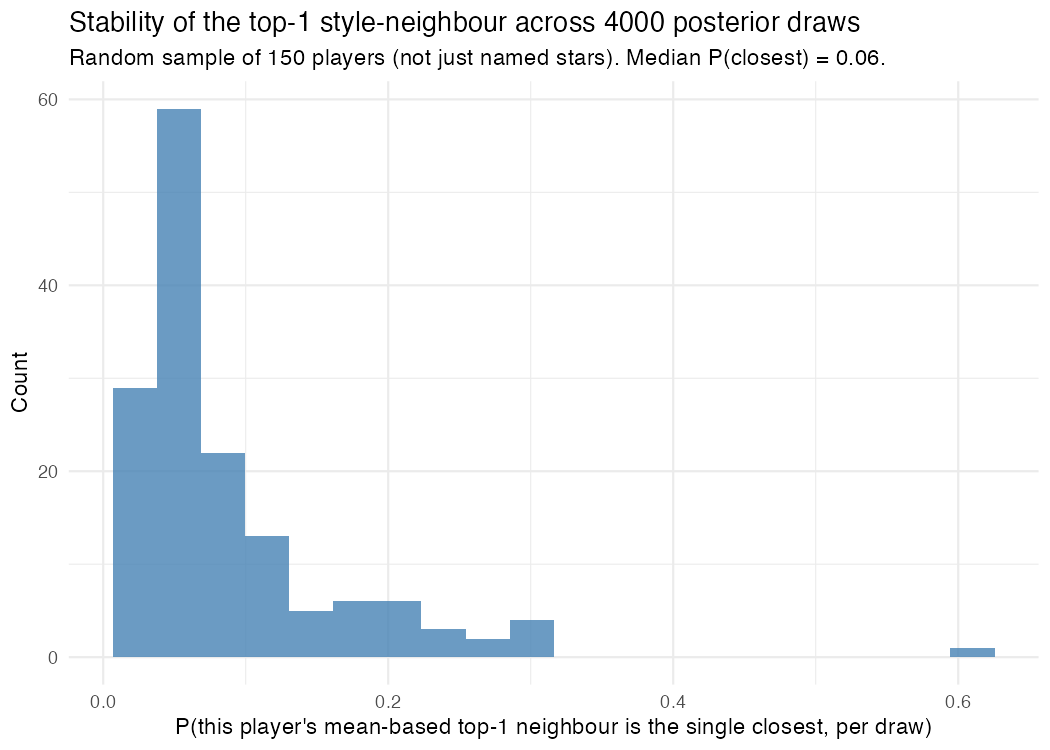
\includegraphics[width=0.7\textwidth]{images/42_population_reliability_hist.png}
\caption{Distribution of $P(\text{closest neighbour stable})$ across a random sample of 150 players.}
\label{fig:population-reliability}
\end{figure}

The result is a sharp contrast with the named case studies: median $P(\text{closest neighbour stable}) = 0.06$,
and only $0.7\%$ of the sampled players reach $P \geq 0.5$. This is not a contradiction of the case-study
findings above --- it is a genuinely different, and important, fact about the shape of the style space. Named
stars occupy comparatively sparse regions near the edges of the player-effect cloud (an unusual combination of
traits has, almost by definition, fewer close rivals), so their single closest neighbour tends to be clearly
separated from the second- and third-closest. Most players, by contrast, sit in denser, more central regions
where many profiles are nearly interchangeable, so no single neighbour dominates and ``the closest neighbour''
is closer to a coin-flip among several candidates. A weak positive relationship with career length (Spearman
$\rho \approx 0.22$ between number of seasons observed and stability) is consistent with more data narrowing the
posterior somewhat, but does not account for the bulk of the effect --- local density in style space is the more
likely primary driver. \textbf{The practical upshot: a ``most similar player'' claim from this model is far
more trustworthy for a stylistically distinctive player than for a stylistically typical one}, and this chapter's
Bayesian treatment is precisely what makes that distinction visible; a point-estimate version of the same metric
would report a single confident-looking neighbour in both cases.

\section{Applications: scouting and recommendations}
\label{sec:results-scouting}

The style/level decomposition of \S\ref{sec:results-similarity} turns directly into a scouting-relevant product:
a shortlist of players who match a target's style at a different output tier, rather than an attempted
like-for-like replacement of an irreplaceable talent. Concretely, the recipe is: fix a target player, take their
top style-neighbours (as in Figure~\ref{fig:style-vs-level-extended}), and read off which of those neighbours
has the largest \emph{level gap} --- that neighbour is a plausible ``cheaper alternative'' candidate, in the
sense of matching shape while differing in the specific output dimension a club may be more willing to accept a
discount on.

This is a style/production tool, not a recruitment decision system, and should be read as one input among many:
market value, age, injury history, contract situation, and league context are not modelled anywhere in this
pipeline, and \S\ref{sec:results-similarity}'s reliability finding is itself a caveat --- the shortlist is far
more trustworthy for a stylistically distinctive target than for a stylistically typical one. Within those
limits, it offers something a purely descriptive scouting report cannot: an explicit, quantified separation of
``how a player plays'' from ``how much they currently produce,'' with honest uncertainty attached to both.

\section{Tactical fit and feature creation}
\label{sec:results-future}

Two further applications were considered and are reported here as scoped future work rather than completed
analysis.

\textbf{Tactical fit.} No team identifier exists anywhere in the current data pipeline (confirmed absent from
both the raw SQL extraction and the model's row-mapping table), so a genuine player-vs-team-system comparison is
not buildable without new data engineering back to the Wyscout source. This ties directly to the team-season
effect $c_{t(i,j),j}$ already identified as a natural modelling extension: adding it would separate
manager/tactical-system effects from stable player identity, and would be the natural foundation for a real
tactical-fit score. Absent that extension, the closest available proxy is simply which of the five archetype
clusters (\S\ref{sec:results-archetypes}) a player belongs to.

\textbf{Feature creation.} Three derived, reporting-only features are proposed but not computed here: a stored
archetype-cluster label per player; a ``style score'' and ``level score'' pair per player, summarising the two
axes of \S\ref{sec:results-similarity} in a single number each; and a soft archetype-membership probability
(e.g.\ from a Gaussian mixture over the canonical factor scores) in place of the current hard $k$-means
assignment, which would let a player be reported as, say, 70\% centre-back / 30\% defensive-midfielder rather
than a single discrete label.
